\section{Cadre idéal}

Nous avons effectué différents tests durant le projet. En utilisant les vidéos fournies sur le site dû MIT. Notre logiciel arrive à obtenir des 
résultats très correct. En effet, par exemple comme on peut le voir sur cette capture d'écran. Après notre magnification réalisée, on retrouve
une fréquence cardiaque d'environ 53 battements par minute (BPM), l'article du MIT lui trouve une fréquence de 54 BPM.  

\begin{figure}[h!]
	\centering
	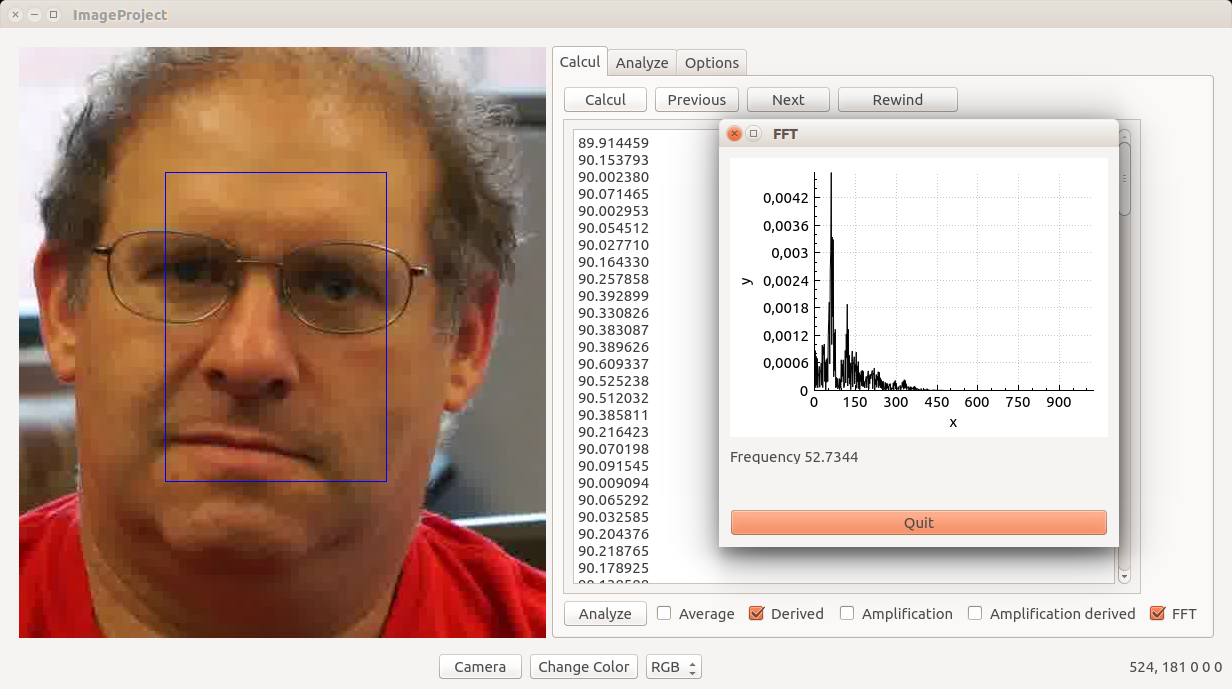
\includegraphics[width=0.9\textwidth]{data/cas-ideal.png}
	\caption{Vidéo source du MIT analysé avec notre logiciel.}
\end{figure}


\section{Webcam}

Avec une webcam, nos résultats sont moins précis, mais sont assez correct pour être utiliser. 

\begin{figure}[h!]
	\centering
	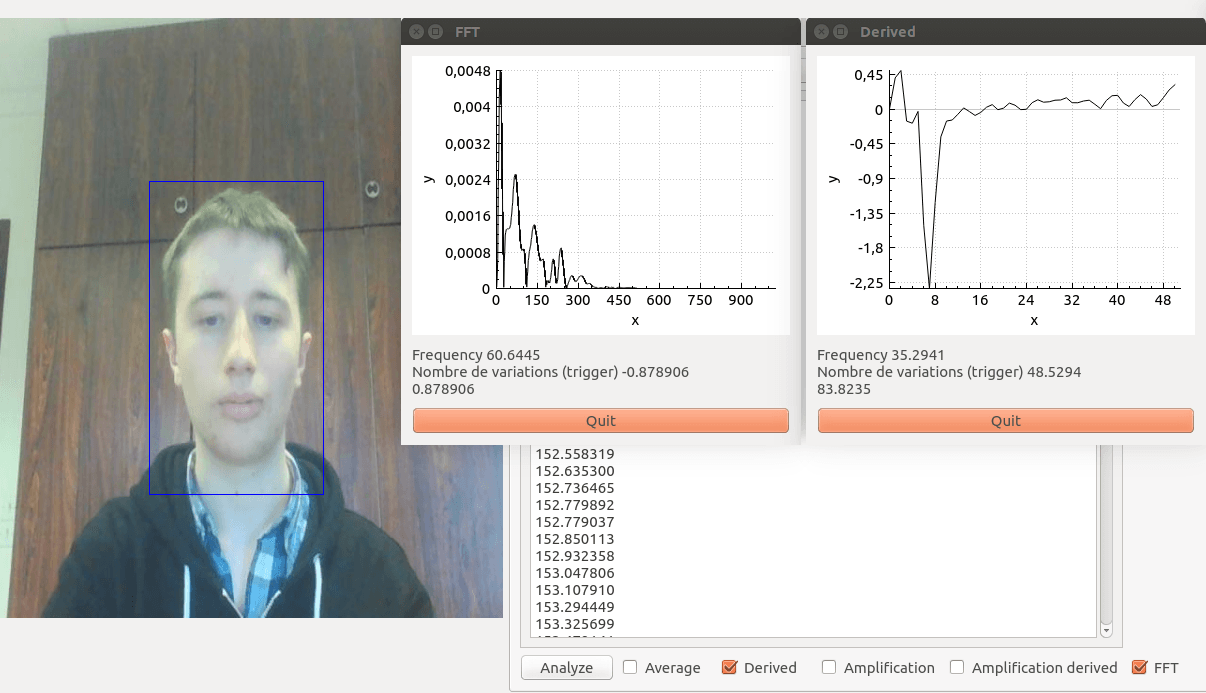
\includegraphics[width=1\textwidth]{data/webcam.png}
	\caption{Vidéo pris par la webcam et analysé avec notre logiciel.}
\end{figure}

\section{Mobile}

\subsection{Android}

Notre plus gros problème a était lors de nos tests sur Android, la stabilité de la vidéo et le nombre de frames capturés.
Actuellement notre application est capable de capturer des frames et appliquer notre algorithme mais nos résultats restent erronées.

\subsection{OpenCV}
	L'utilisation d'une FFT et d'un Trigger permet de mieux différencier l'homme de la photo. Même si les résultats sont meilleurs il reste de nombreuses erreurs et le temps de calcul est beaucoup plus long.G

\section{Bilan}

Notre différenciation entre un humain et une photo fonctionne correctement dès lors où la stabilité est assurée. En effet, prenons Android, nous arrivons
à capturer plus de frames qu'en utilisant OpenCV, toutefois le tracking d'OpenCV est plus efficace. De ce fait, malgré une meilleure capture sous Android 
comme la stabilité est plus mauvaise, nos résultats sont moins bons. Mais à contrario, lorsqu'on utilise l'application réalisée avec OpenCV, le nombre d'images
capturé est seulement de 20 pour 4 secondes, avec si peu d'images à traiter notre magnification n'est pas correcte. C'est seulement au bout de 10 secondes
lorsqu'on capture entre 50 à 70 frames qu'on a des résultats cohérents. 

